\documentclass[11pt]{article}
\usepackage[margin=1in]{geometry}
\usepackage[T1]{fontenc}
\usepackage{lmodern}
\usepackage{amsmath,amsthm,booktabs,hyperref,microtype,graphicx,array}
\usepackage[section]{placeins}
\hypersetup{hidelinks}
\makeatletter\let\tableinput\@@input\makeatother
% Generated; do not edit. ATT&CK mitigation gaps.
\newcommand{\GapComparable}{15}
\newcommand{\GapDipFloor}{18.4}
\newcommand{\GapDipFloorBefore}{23.0}
\newcommand{\GapDipStage}{impact}
\newcommand{\GapDipTech}{T1485}
\newcommand{\GapDipTechName}{Data Destruction}
\newcommand{\GapDipVersion}{16.1}
\newcommand{\GapFirstDate}{2019-07}
\newcommand{\GapFirstMit}{39}
\newcommand{\GapFirstShare}{25.0}
\newcommand{\GapFirstSingle}{66}
\newcommand{\GapFirstStages}{8}
\newcommand{\GapFirstTech}{244}
\newcommand{\GapFirstUnc}{61}
\newcommand{\GapFirstVersion}{5.2}
\newcommand{\GapFloorEvents}{6}
\newcommand{\GapFloorFirstKOne}{14.7}
\newcommand{\GapFloorGrowth}{1.56}
\newcommand{\GapFloorLastKFour}{5.1}
\newcommand{\GapFloorLastKOne}{23.0}
\newcommand{\GapFloorRatio}{9.3}
\newcommand{\GapFloorRepairedLastKOne}{2.5}
\newcommand{\GapInhFirstUnc}{61}
\newcommand{\GapInhFloor}{18.4}
\newcommand{\GapInhFloorFirst}{14.7}
\newcommand{\GapInhFloorGrowth}{1.25}
\newcommand{\GapInhGrowthPct}{21}
\newcommand{\GapInhRepFive}{12}
\newcommand{\GapInhRepTen}{3}
\newcommand{\GapInhStages}{9}
\newcommand{\GapInhUnc}{74}
\newcommand{\GapLastDate}{2026-08}
\newcommand{\GapLastMit}{42}
\newcommand{\GapLastShare}{19.0}
\newcommand{\GapLastSingle}{135}
\newcommand{\GapLastStages}{10}
\newcommand{\GapLastTech}{601}
\newcommand{\GapLastUnc}{114}
\newcommand{\GapLastVersion}{19.2}
\newcommand{\GapMinShare}{17.4}
\newcommand{\GapMinShareVersion}{15.1}
\newcommand{\GapParamLowFloor}{0.02}
\newcommand{\GapParamMidFloor}{1.1}
\newcommand{\GapParamStrongFloor}{12.3}
\newcommand{\GapParamStrongRep}{1}
\newcommand{\GapParamSubsetAll}{every}
\newcommand{\GapParamWeakFloor}{32.7}
\newcommand{\GapParamWeakRep}{infeasible}
\newcommand{\GapParentsUncLast}{48}
\newcommand{\GapParentsUncSub}{40}
\newcommand{\GapPlaceholderUnc}{111}
\newcommand{\GapPreSubShare}{25.6}
\newcommand{\GapReleases}{19}
\newcommand{\GapRepFiveOne}{26}
\newcommand{\GapRepFiveOneStages}{7}
\newcommand{\GapRepHistFirst}{5}
\newcommand{\GapRepHistMax}{9}
\newcommand{\GapRepHistMaxVersion}{15.1}
\newcommand{\GapRepOneFour}{36}
\newcommand{\GapRepOneOne}{infeasible}
\newcommand{\GapRepTenOne}{6}
\newcommand{\GapRepTenOneStages}{4}
\newcommand{\GapRepWeakFiveOne}{infeasible}
\newcommand{\GapRepWeakTenOne}{36}
\newcommand{\GapRiseFloor}{23.0}
\newcommand{\GapRiseStage}{execution}
\newcommand{\GapRiseTech}{T1059.012}
\newcommand{\GapRiseTechName}{Hypervisor CLI}
\newcommand{\GapRiseVersion}{17.1}
\newcommand{\GapSplitFloorKOne}{20.7}
\newcommand{\GapSplitStages}{11}
\newcommand{\GapStages}{12}
\newcommand{\GapSubShare}{19.6}
\newcommand{\GapTechGrowthPct}{146}
\newcommand{\GapUncGrowthPct}{87}
\newcommand{\GapWorstCountStage}{defense-evasion}
\newcommand{\GapWorstCountUnc}{43}
\newcommand{\GapWorstSharePct}{71}
\newcommand{\GapWorstShareStage}{discovery}
\newcommand{\GapWorstShareTotal}{49}
\newcommand{\GapWorstShareUnc}{35}

\newtheorem{proposition}{Proposition}

\title{Uncoverable by Design: Seven Years of Mitigation Gaps in MITRE ATT\&CK,\\
the Certification Floor They Impose, and Their Minimal Repair}
\author{}
\date{2026-09-23 (preprint draft, version 0.2.0)}

\begin{document}
\maketitle

\begin{abstract}
MITRE ATT\&CK is the reference knowledge base for threat-informed defense, and
control-selection tools read its \texttt{mitigates} relationships to decide which
controls counter which adversary techniques. Using the latest patch of every comparable
Enterprise release from v\GapFirstVersion{} (\GapFirstDate) to v\GapLastVersion{}
(\GapLastDate), we measure how many post-compromise ransomware kill-chain techniques
ATT\&CK maps to no mitigation. The kill chain grew from \GapFirstTech{} to \GapLastTech{}
techniques while real mitigations grew from \GapFirstMit{} to \GapLastMit; techniques
with no mitigation rose from \GapFirstUnc{} to \GapLastUnc{} (+\GapUncGrowthPct\%) when
each technique is judged by its own mapping, and from \GapInhFirstUnc{} to \GapInhUnc{}
(+\GapInhGrowthPct\%) when sub-techniques inherit their parent's mitigations. Because an
adaptive adversary can route through an unmitigated technique, these gaps impose a
\emph{certification floor}: when the per-technique base rate is only known to lie in
$[0.5,0.9]$ and control effectiveness is interval-uncertain, no portfolio of ATT\&CK
mitigations can be certified to keep the worst-case probability of a clinical-service
outage in our hospital-ransomware model below \GapFloorLastKOne\% today
(\GapInhFloor\% with inheritance; \GapFloorFirstKOne\% in \GapFirstDate). The level is
assumption-driven --- it is \GapParamMidFloor\% if the base rate is at most 0.7 --- but
the floor factorises into a base-rate term and a coverage term, so its
\GapFloorGrowth-fold rise across releases does not depend on the base rate. We also
solve, exactly, the \emph{minimal coverage repair}: in v\GapLastVersion{}, mapping a
mitigation to \GapRepTenOne{} specific techniques (\GapInhRepTen{} with inheritance)
makes a 10\% certificate attainable. Gaps between ATT\&CK techniques and mapped controls
have been measured before in a single snapshot; the longitudinal series, the floor and
the exact repair are, to our knowledge, new, and the underlying arguments are elementary.
\end{abstract}

\section{Introduction}
ATT\&CK~\cite{strom2018} catalogues adversary behaviour as tactics and techniques and
links each technique to the mitigations that counter it. Those links are the defensive
half of the model: coverage heatmaps, control-gap assessments and automated
control-selection tools all consume them~\cite{roy2023sok,alsada2024}. A technique with
no mitigation cannot be covered by any portfolio of mapped mitigations, however large,
so every tool that reasons only from the mapping inherits it as a permanent gap.

This paper asks four questions of that defensive half, using real ATT\&CK data across
releases. \textbf{(Q1)} How many ransomware kill-chain techniques have no mitigation, and
is the gap closing? \textbf{(Q2)} What lower bound on certifiable worst-case residual
risk do those gaps force on \emph{any} defense built from ATT\&CK mitigations?
\textbf{(Q3)} What is the smallest set of techniques that would need a mitigation for a
given guarantee to become attainable, and which are they? \textbf{(Q4)} Which of these
answers depend on counting conventions and model parameters, and which do not?

\paragraph{Contributions.} (i) A longitudinal measurement of mitigation coverage over
\GapComparable{} comparable Enterprise releases (\GapFirstDate--\GapLastDate), handling
the mitigation restructure, the arrival of sub-techniques, the v19 split of Defense
Evasion, and placeholder mitigations explicitly, under two sub-technique conventions.
(ii) A distribution-free certification floor per release
(Proposition~\ref{prop:floor}) and a factorisation showing that its growth across
releases is free of the base rate (Proposition~\ref{prop:base}). (iii) An exact minimal
repair, justified by a structural result that partial repair of a stage is worthless
(Proposition~\ref{prop:repair}), with the resulting technique list. (iv) Sensitivity of
every headline to conventions and parameters. All data, code and tables are released
with hash-pinned provenance.

\section{Background and related work}
ATT\&CK's design is documented by its authors~\cite{strom2018}. Two surveys systematise
the research that uses it~\cite{roy2023sok,alsada2024}; they track how the framework has
grown and how it is applied, but do not measure the techniques it leaves without a
mitigation over time. Closest to our work, Rahman and Williams~\cite{rahman2022} study
how far NIST SP~800-53 controls mitigate 188 ATT\&CK techniques through the Center for
Threat-Informed Defense's control mapping, in one snapshot; we instead use ATT\&CK's own
mitigation objects, follow them across seven years of releases, and turn the gaps into a
bound and a repair problem. Vendor ``ATT\&CK coverage'' reports concern \emph{detection}
coverage of a product, not the knowledge base's own mitigation mapping. Our floor uses a
sharp distribution-free bound on the probability that at least $k$ of $n$ dependent
events occur, in closed form (a Fr\'echet-type bound; proof and verification in the
accompanying note \texttt{study/KOFN\_THEOREM.md}). Our search for prior work (arXiv and
web search for ATT\&CK together with mitigation coverage, mitigation gaps, unmitigated
techniques and control mapping, September 2026) found no longitudinal measurement of
unmitigated techniques; this is an absence of evidence, not proof of novelty.

\section{Data and definitions}
\paragraph{Releases.} We take the latest patch of every major Enterprise release,
\GapReleases{} in all, from MITRE's official STIX repository; raw bundles are
hash-verified and compact extracts are released. A release is \emph{comparable} if its
mitigations use the generalised \texttt{M\#\#\#\#} identifiers, every kill-chain stage is
populated, and T1486 (Data Encrypted for Impact) is present. Releases v1--v4 fail the
first test --- their mitigations were technique-specific objects, one per technique ---
so the series begins at v\GapFirstVersion.

\paragraph{Kill chain and coverage.} The kill chain is the post-compromise ransomware
tactics from Initial Access to Impact, \GapStages{} stages in all. A \emph{real
mitigation} is any active mitigation except the placeholders M1055 \emph{Do Not
Mitigate} and M1056 \emph{Pre-compromise}, which record that no preventive control
applies. A kill-chain technique is \emph{uncovered} if it has no real mitigation. By
default each technique, including each sub-technique, is judged by its own mapping; the
\emph{inheritance} convention instead lets an unmapped sub-technique inherit its parent's
mitigations, as a coverage tool that rolls sub-techniques up to parents would.

\paragraph{Structural breaks.} Sub-techniques arrive in v7, so technique counts jump; we
report parent-technique counts alongside. ATT\&CK v19 splits Defense Evasion into
Stealth and Defense Impairment; a crosswalk maps both to one stage so the kill-chain
model is constant across releases, and we report the split as a sensitivity.

\section{The certification floor}
Following our certificate framework, each technique $t$ succeeds per attempt with base
rate $b$, and each deployed mitigation $m$ that covers $t$ multiplies that by $1-e_m$.
Both are interval-uncertain: $b\in[0.5,0.9]$, and each $e_m$ has lower end $0.20$,
except the evidence-tightened MFA control M1032 with lower end $0.85$. A certificate must
hold over the whole uncertainty set, so it is decided at the worst corner ($b=0.9$,
every $e_m$ at its lower end). An \emph{adaptive} adversary best-responds to the defense
by using, at each stage, the technique with the largest residual; clinical reachability
is the product of the \GapStages{} stage maxima, and the probability that at least $k$
of four clinical services suffer sustained outage is bounded by the sharp $k$-of-$n$
bound at marginals proportional to it.

\begin{proposition}[Floor]\label{prop:floor}
Over all portfolios of real ATT\&CK mitigations, adaptive reachability is minimised by
deploying every mitigation, and every stage containing an uncovered technique has
factor exactly $b$.
\end{proposition}
\begin{proof}
Deploying $m$ multiplies each residual it touches by $1-e_m\le 1$ and leaves the rest
unchanged, so residuals, stage maxima and their product are non-increasing in the
portfolio; the full portfolio is a minimiser. An uncovered technique has residual $b$
under every portfolio, and every residual is at most $b$, so its stage maximum is $b$.
\end{proof}

Hence a certificate ``$\Pr(\ge k$ services down$)\le\varepsilon$'' is attainable with
ATT\&CK mitigations only if the floor is at most $\varepsilon$. The floor's level is
driven by $b$, but its change across releases is not:

\begin{proposition}[Base-rate factorisation]\label{prop:base}
For fixed effectiveness values, the floor reachability of a release is
$F(b)=b^{n}\,C$, where $n$ is the number of stages and $C$ depends only on the release's
coverage and the effectiveness values. Hence the ratio of the floors of two releases
with the same stages does not depend on $b$, and neither does the ratio of their
$k$-of-$n$ floors while both are below one.
\end{proposition}
\begin{proof}
Each residual is $b$ times a product of $(1-e_m)$ factors, so each stage maximum is $b$
times the maximum of those products, and $F$ is $b^n$ times the product of the latter.
The sharp $k$-of-$n$ bound is a minimum of linear functions of the marginals and $1$, so
it is positively homogeneous in $F$ until it reaches one.
\end{proof}

\section{Minimal coverage repair}
Suppose a set $R$ of uncovered techniques each gains one mitigation of worst-corner
effectiveness $e_{\mathrm{new}}$. We seek the smallest $|R|$ making the floor at most
$\varepsilon$. Let $U_s$ be the uncovered techniques of stage $s$.

\begin{proposition}[Whole-stage repair]\label{prop:repair}
For any feasible $R$, the set $R'=\bigcup\{U_s : U_s\subseteq R\}$ is feasible, has
$|R'|\le|R|$, and yields the same floor. Hence an optimal repair is a union of whole stage
gap sets.
\end{proposition}
\begin{proof}
By Proposition~\ref{prop:floor}, a stage keeps factor $b$ while any member of $U_s$ is
unrepaired, so only stages with $U_s\subseteq R$ change. $R'\subseteq R$ completes
exactly those stages, and the techniques in $R\setminus R'$ lie in stages that stay at
$b$; so the floor is unchanged.
\end{proof}

With \GapStages{} stages, enumerating stage subsets and costing each union of gap sets
--- counting a technique shared by several tactics once --- solves the problem exactly.
We verify the procedure against brute force over every subset of uncovered techniques on
instances with shared techniques.

\section{Results}
\paragraph{Coverage is not keeping pace.} Figure~\ref{fig:coverage} (left) and
Table~\ref{tab:release}: between v\GapFirstVersion{} and v\GapLastVersion{} the kill chain
grew by \GapTechGrowthPct\% (\GapFirstTech{} to \GapLastTech{} techniques) while real
mitigations grew only from \GapFirstMit{} to \GapLastMit. Uncovered techniques rose from
\GapFirstUnc{} to \GapLastUnc{} (+\GapUncGrowthPct\%). As a share, the gap fell when
sub-techniques arrived (\GapPreSubShare\% to \GapSubShare\%), bottomed at
\GapMinShare\% in v\GapMinShareVersion, and has risen since to \GapLastShare\%; among
parent techniques, uncovered ones rose from \GapParentsUncSub{} in v7 to
\GapParentsUncLast. Thin coverage --- techniques with exactly one mitigation --- doubled,
from \GapFirstSingle{} to \GapLastSingle. The gap is concentrated (Table~\ref{tab:tactic}):
\GapWorstSharePct\% of \GapWorstShareStage{} techniques (\GapWorstShareUnc{} of
\GapWorstShareTotal) and \GapWorstCountUnc{} \GapWorstCountStage{} techniques have no
mitigation, and \GapLastStages{} of \GapStages{} kill-chain stages contain at least one
uncovered technique (\GapFirstStages{} in v\GapFirstVersion). Much of the growth is
sub-techniques whose parent is mapped: with inheritance, uncovered techniques rose from
\GapInhFirstUnc{} to \GapInhUnc{} (+\GapInhGrowthPct\%) and \GapInhStages{} stages
contain a gap. The direction holds under both conventions; the size does not.

\paragraph{The floor has risen.} Figure~\ref{fig:coverage} (right): no portfolio can be
certified to keep the worst-case probability that at least one of the four clinical
services suffers sustained outage below \GapFloorFirstKOne\% with v\GapFirstVersion{}
mitigations and \GapFloorLastKOne\% with v\GapLastVersion{} mitigations
(\GapFloorLastKFour\% for all four services at once). With inheritance the latest floor
is \GapInhFloor\% (a \GapInhFloorGrowth-fold rise instead of \GapFloorGrowth-fold). The
floor is set stage by stage by a single \emph{binding} technique --- the adversary's best
route --- so it moves only when one mapping decision changes a binding technique; across
the comparable releases that happened \GapFloorEvents{} times (Table~\ref{tab:changes}).
The sharpest pair: in v\GapDipVersion{} the floor fell from \GapDipFloorBefore\% to
\GapDipFloor\% because \GapDipTechName{} (\GapDipTech), which bound the \GapDipStage{}
stage, gained further mitigations; in v\GapRiseVersion{} a single newly added technique
with no mitigation, \GapRiseTechName{} (\GapRiseTech), opened a gap in \GapRiseStage{}
and returned the floor to \GapRiseFloor\%. A single unmitigated technique was enough to
cancel that improvement. If every gap were closed with a mitigation as strong as the
existing ones, the floor would fall to \GapFloorRepairedLastKOne\% --- a
\GapFloorRatio-fold reduction.

\paragraph{The minimal repair is small for moderate targets.} Figure~\ref{fig:repair}:
in v\GapLastVersion, mitigating \GapRepTenOne{} techniques across \GapRepTenOneStages{}
stages (Table~\ref{tab:repair}) makes a 10\% single-service certificate attainable; a 5\%
certificate needs \GapRepFiveOne{} techniques across \GapRepFiveOneStages{} stages; a 1\%
certificate on all four services needs \GapRepOneFour; and a 1\% single-service
certificate is \GapRepOneOne{} even with every gap closed, because the remaining floor is
set by thinly covered techniques. With inheritance the 10\% and 5\% repairs need
\GapInhRepTen{} and \GapInhRepFive{} techniques. The 10\% repair cost was
\GapRepHistFirst{} in v\GapFirstVersion, peaked at \GapRepHistMax{} in
v\GapRepHistMaxVersion, and is \GapRepTenOne{} today. At $e_{\mathrm{new}}=0.2$ and
$0.5$ the repair costs are identical, because a repaired stage then binds on its weakest
existing mapping; a weaker new mitigation ($e_{\mathrm{new}}=0.1$) raises the 10\%
repair to \GapRepWeakTenOne{} techniques and makes the 5\% certificate
\GapRepWeakFiveOne.

\paragraph{Levels are assumption-driven; the trend is not.} Table~\ref{tab:params}
varies the upper end of the base-rate interval and the lower end of mitigation
effectiveness. The level of the floor moves by orders of magnitude: it is
\GapParamMidFloor\% at $b=0.7$ and \GapParamLowFloor\% at $b=0.5$, and at $b=0.9$ it is
\GapParamWeakFloor\% or \GapParamStrongFloor\% as effectiveness is weakened or
strengthened. Below $b=0.9$ no repair is needed even for a 5\% certificate; at $b=0.9$
with stronger effectiveness a 10\% certificate needs \GapParamStrongRep{} technique,
drawn from the default list (\GapParamSubsetAll{} feasible setting needs only techniques
from that list). By Proposition~\ref{prop:base}, however, the \GapFloorGrowth-fold growth
of the floor between v\GapFirstVersion{} and v\GapLastVersion{} holds for every $b$ at
fixed effectiveness. The robust findings are thus the direction of the gap, the factor
by which it has raised the floor, and which techniques bind; the absolute percentages
are conditional on the uncertainty set.

\paragraph{Other conventions.} Counting the placeholder mitigations as controls ---
as a literal reading of the \texttt{mitigates} relationships does --- reports
\GapPlaceholderUnc{} rather than \GapLastUnc{} uncovered techniques in
v\GapLastVersion{} and leaves the floor unchanged. Treating v19's Stealth and Defense
Impairment as separate stages gives \GapSplitStages{} gap stages and a floor of
\GapSplitFloorKOne\% (an extra stage multiplies in another factor below one).

\begin{figure}[t]\centering
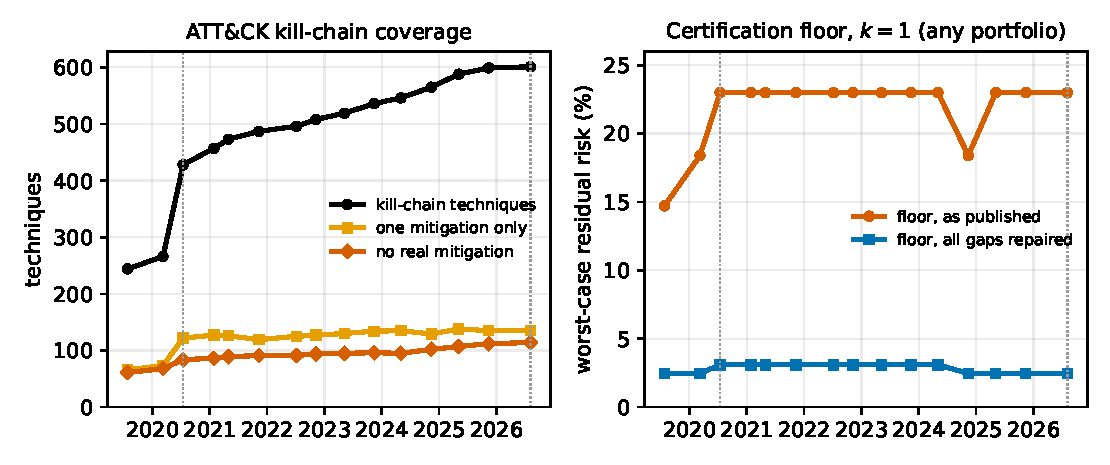
\includegraphics[width=\linewidth]{figure_coverage_floor.pdf}
\caption{Left: kill-chain techniques, techniques with a single mitigation, and techniques
with no real mitigation, per release. Right: the certification floor on the worst-case
probability of at least one clinical-service outage ($b=0.9$), as published and with
every gap repaired. Dotted lines: sub-techniques (v7) and the Defense Evasion split
(v19).}\label{fig:coverage}
\end{figure}

\begin{figure}[t]\centering
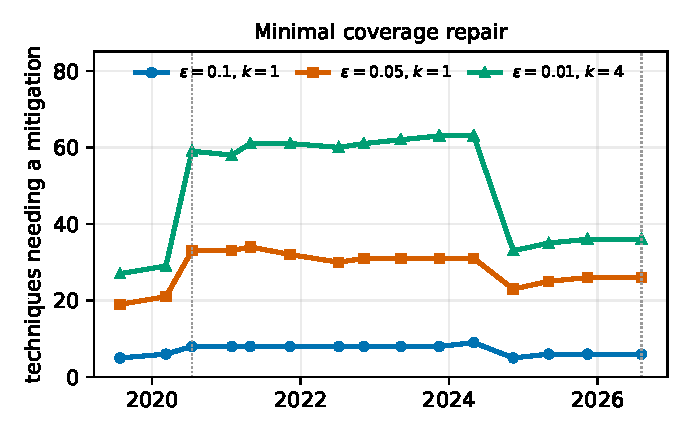
\includegraphics[width=0.62\linewidth]{figure_repair.pdf}
\caption{Fewest techniques needing a mitigation for each certificate to become
attainable, per release ($e_{\mathrm{new}}=0.2$). The target $\varepsilon=0.05$, $k=2$
coincides with $\varepsilon=0.10$, $k=1$ and is omitted. Dotted lines as in
Figure~\ref{fig:coverage}.}\label{fig:repair}
\end{figure}

\begin{table}[t]\centering\small
\caption{Per release: kill-chain techniques, real mitigations, uncovered techniques
(share, \%), techniques with a single mitigation, stages containing an uncovered
technique, the floor for $k{=}1$ (\%), and the minimal repair for $\varepsilon{=}0.10$,
$k{=}1$.}\label{tab:release}
\begin{tabular}{@{}llrrrrrrr@{}}\toprule
Ver. & Date & Tech. & Mit. & Uncovered & One mit. & Gap st. & Floor & Repair\\\midrule
\tableinput table_gaps_release_rows.tex
\bottomrule\end{tabular}
\end{table}

\begin{table}[t]\centering\small
\caption{Uncovered/total techniques per kill-chain tactic, first and latest comparable
release, and the latest share (\%). The Impact row counts every Impact technique; the
floor's impact stage uses the four clinical-impact techniques, all of which are
mitigated. Defense Evasion in v\GapLastVersion{} is Stealth $\cup$ Defense
Impairment.}\label{tab:tactic}
\begin{tabular}{@{}lrrr@{}}\toprule
Tactic & v\GapFirstVersion & v\GapLastVersion & Share\\\midrule
\tableinput table_gaps_tactic_rows.tex
\bottomrule\end{tabular}
\end{table}

\begin{table}[t]\centering\small
\caption{Parameter sensitivity in v\GapLastVersion: upper end of the base-rate interval
$b$, lower end of mitigation effectiveness $e$, the floor for $k{=}1$ (\%), and the
minimal repair for a 10\% and a 5\% single-service certificate.}\label{tab:params}
\begin{tabular}{@{}rrrrr@{}}\toprule
$b$ & $e$ & Floor & Repair 10\% & Repair 5\%\\\midrule
\tableinput table_gaps_param_rows.tex
\bottomrule\end{tabular}
\end{table}

\begin{table}[t]\centering\small
\caption{Every change in the floor across comparable releases: the stage whose factor
changed and the technique that binds it (the adaptive adversary's best route) before and
after. A factor of 0.900 means the stage contains a technique with no
mitigation.}\label{tab:changes}
\begin{tabular}{@{}llr>{\raggedright}p{3.7cm}>{\raggedright\arraybackslash}p{3.7cm}@{}}\toprule
Ver. & Stage & Factor & Binding before & Binding after\\\midrule
\tableinput table_gaps_changes_rows.tex
\bottomrule\end{tabular}
\end{table}

\begin{table}[t]\centering\small
\caption{The minimal repair in v\GapLastVersion{} for a 10\% single-service certificate:
the techniques that would need a mitigation.}\label{tab:repair}
\begin{tabular}{@{}lll@{}}\toprule
Technique & Name & Stage\\\midrule
\tableinput table_gaps_repair_rows.tex
\bottomrule\end{tabular}
\end{table}

\section{Discussion}
For the maintainers of ATT\&CK, the repair list is a candidate authoring agenda: a
handful of mitigation mappings would change what any ATT\&CK-driven defense can be
certified to achieve under our model, whereas the long tail of Discovery techniques ---
routine enumeration of the environment --- is where preventive mitigations are hardest
to write and where detection must carry the load. For builders of control-selection and
coverage tools, every uncovered technique is a gap inherited by construction; tools
should surface it rather than report full coverage, and should state which sub-technique
convention they use, since it changes the count substantially. For defenders, the floor
is a reason to pair preventive portfolios with detection and response for the uncovered
techniques, and the thin-coverage count identifies where a single failed control leaves a
technique effectively unmitigated.

\section{Limitations}
\paragraph{Mapping, not reality.} ``No mitigation in ATT\&CK'' measures the knowledge
base's mitigation \emph{mapping}, not the absence of any real-world defense; detections
and vendor controls exist for many uncovered techniques, and a technique may lack a
mapping because no \emph{preventive} control is appropriate. Coverage counts inherit
ATT\&CK's editorial choices, including when behaviours are split into sub-techniques.

\paragraph{Levels are assumption-driven.} The floor's level depends on the base-rate
interval, the effectiveness intervals, a stage-based kill-chain model and a synthetic
hospital-ransomware impact model; Table~\ref{tab:params} shows it can fall below 1\%.
It is a bound under those assumptions, not a measured incident rate, and we do not
validate it against incidents. Only its relative change is free of the base rate.

\paragraph{Required tactics.} We assume every kill-chain tactic must be traversed.
Requiring fewer tactics removes factors below one from the product, so it can only raise
the floor: ours is a lower bound for any subset of required tactics under the same
parameters.

\paragraph{Counting conventions.} The size of the growth in uncovered techniques depends
on whether sub-techniques inherit their parent's mitigations
(+\GapUncGrowthPct\% versus +\GapInhGrowthPct\%). Placeholder mitigations and the v19
split are handled by stated rules, with alternatives reported.

\paragraph{Adversary.} The adaptive adversary is worst case: it knows the defense and
always uses the easiest technique at each stage. Real adversaries are less informed, so
the floor bounds what can be \emph{certified}, not what is typically experienced.

\paragraph{Repair.} The repair assumes a new mitigation behaves like the existing ones;
we report sensitivity to its strength. Writing an effective mitigation for a technique
may be infeasible, which the count does not capture.

\paragraph{Artifact and AI use.} Per-release extracts with SHA-256 provenance, the
analysis code, tests (including exact agreement with an independent implementation of
the floor and a brute-force check of the repair), and every table are released; all
numbers in this paper are generated from committed tables. The analysis code and draft
text were produced with the assistance of an AI system (Claude); all results are
reproduced by automated tests.

\begin{thebibliography}{9}
\bibitem{strom2018} B.~E. Strom et al.
\newblock MITRE ATT\&CK: Design and Philosophy.
\newblock MITRE Technical Report, 2018 (revised 2020).
\bibitem{roy2023sok} S.~Roy, E.~Panaousis, C.~Noakes, A.~Laszka, S.~Panda, and G.~Loukas.
\newblock SoK: The MITRE ATT\&CK Framework in Research and Practice.
\newblock arXiv:2304.07411, 2023.
\bibitem{alsada2024} B.~Al-Sada, A.~Sadighian, and G.~Oligeri.
\newblock MITRE ATT\&CK: State of the Art and Way Forward.
\newblock \emph{ACM Computing Surveys}, 2024. arXiv:2308.14016.
\bibitem{rahman2022} M.~R. Rahman and L.~Williams.
\newblock An investigation of security controls and MITRE ATT\&CK techniques.
\newblock arXiv:2211.06500, 2022.
\end{thebibliography}

\end{document}
